\documentclass[11pt]{article}
% Horizontal Magnetic Dipole over a lossy half-space
\usepackage[utf8]{inputenc} % Use it to include other characters than ABC
\usepackage[cmex10]{amsmath}
\usepackage{mdwmath}
\usepackage{mdwtab}
\usepackage{hyperref}
\usepackage{physics} % For using the oridnary derivative nomenclature
\usepackage{datetime} % Insert date and time
\usepackage[letterpaper, margin=1in]{geometry}
\usepackage{graphicx}
\usepackage{pgfplots}
\usepackage{tikz}
\usepackage{standalone}
\usepackage[americanresistors,americaninductors]{circuitikz} % For circuit elements
\usepackage{tikz-dimline} % For dimensional drawing
\usetikzlibrary{positioning}
\usetikzlibrary{arrows}
\usepackage{subfig}
% The following is done to hide ugly color boces around the links
\usepackage{xcolor}
\hypersetup{
colorlinks,
linkcolor={red!50!black},
citecolor={blue!50!black},
urlcolor={blue!80!black}
}
% \usepackage{pdfsync} % use to back search tex lines from pdf
% pdflatex -synctex=-1
% \usepackage{mathptmx} % Times new Roman

% ------------------------------- Useful Tricks Learnt
% Use ={}& to align subequations to the left
% Use = for single equations
% Put comments % in between the lines in order to avoid forming a new paragraph.
% To enter special characters into Inkspace figures, use Ctrl+U and then enter       the unicode. e.g., for \times symbol, the unicode is U+0D7. So the key entry would be Ctrl+U U+0d7 and then press enter.
%
% ----------------- To compile with references use the following order in Shell"
% 1. pdflatex filename.tex
% 2. bibtex filename (no extension)
% 3. bibtex filename (no extension)
% 4. pdflatex filename.tex
% -----------------

% Personal definitions
% Operators
\renewcommand{\v}[1]{\mathbf{#1}} % vectors
\newcommand{\ti}[1]{\tilde{#1}} % spectral representation

% Symbols
\renewcommand{\O}{\omega}  % omega
\newcommand{\E}{\varepsilon}  % epsilon
\renewcommand{\u}{\mu}  % mu
\newcommand{\p}{\rho}  % rho
\newcommand{\x}{\times}  % times
\renewcommand{\inf}{\infty}  % infinity
\newcommand{\infint}{\int\limits_{-\inf}^\inf} % integral by R
\newcommand{\del}{\nabla}  % nabla operator
\renewcommand{\^}{\hat}  % unit vector


\begin{document}
\title{\textsc{Horizontal Electric Dipole}\\}
\date{\footnote{Last Modified: \currenttime, \today.}}
% \maketitle



\section{No PEC backing}

The computed zeros for the structure with no PEC backing as shown in \ref{fig:structure} are obtained through Halley's method performed on the denominator expression:

\begin{align}
  \mathcal D = 1 -\overleftarrow{\Gamma_2} \overrightarrow{\Gamma_2} e^{-2jk_{z2} d_{1}}
  \label{eq:D}
\end{align}

\begin{figure}[h!]
  \centering
  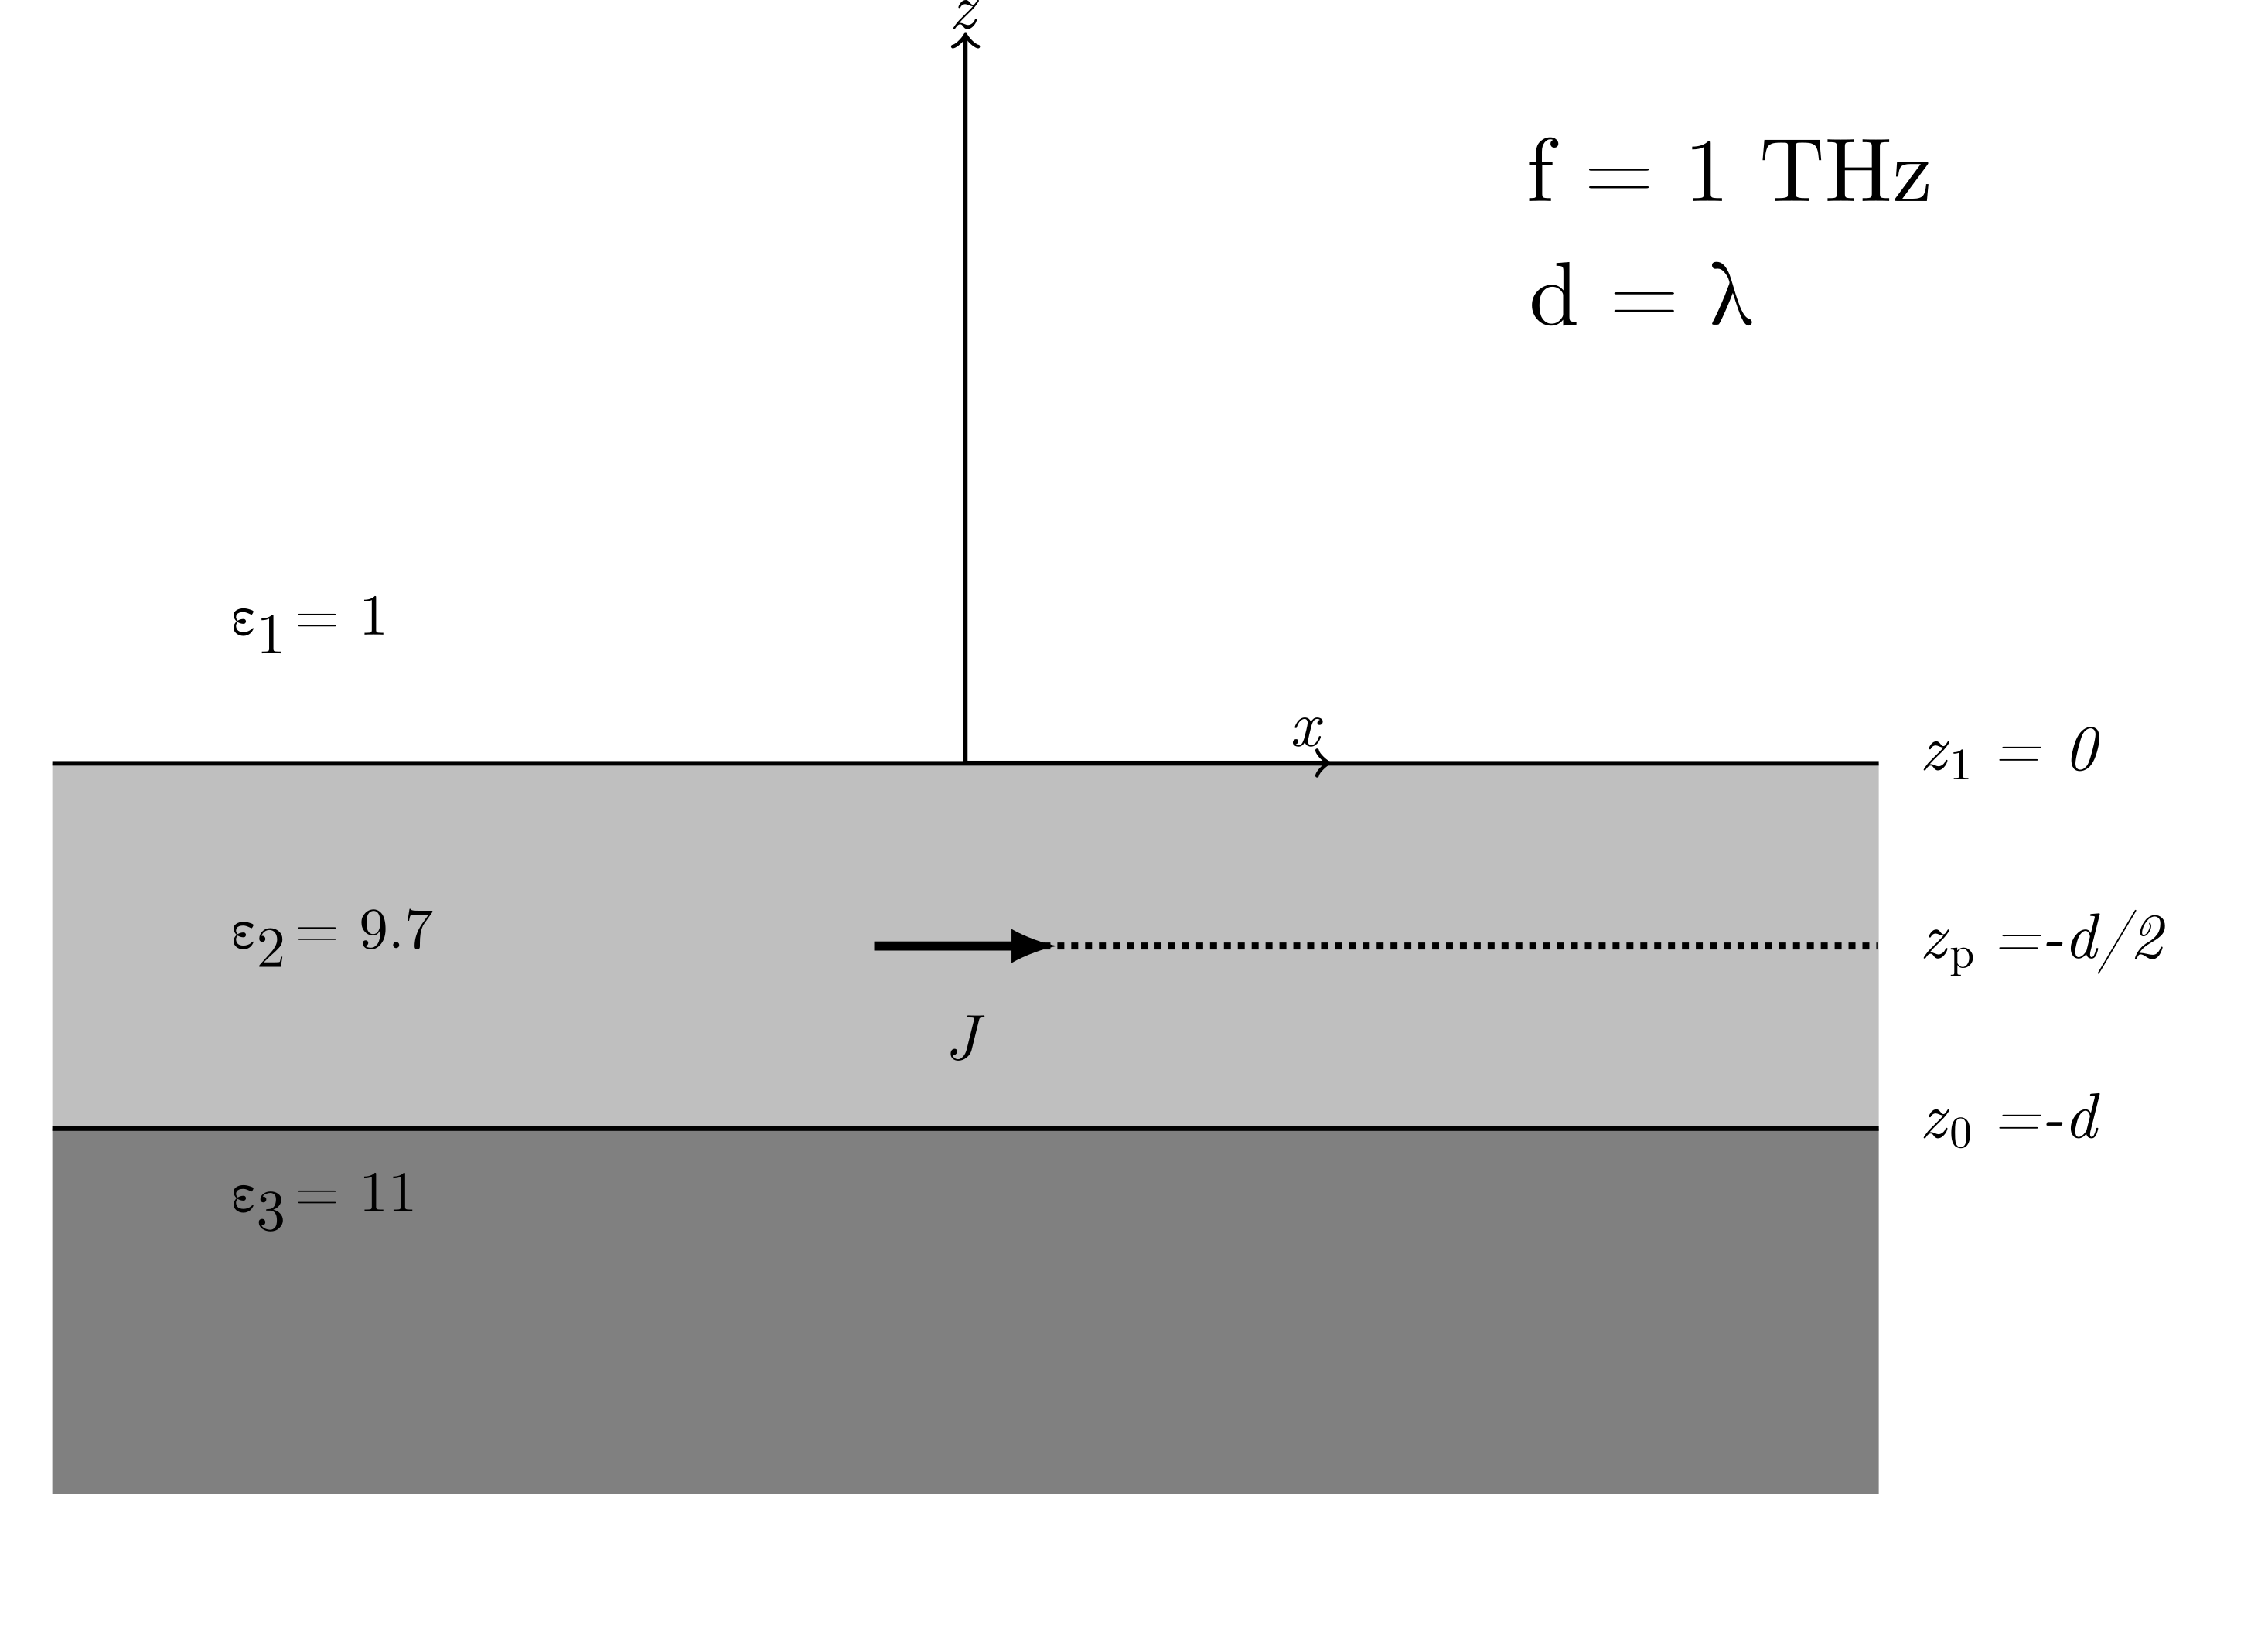
\includegraphics[width=.85\textwidth]{structure_with_no_PEC_Backing}
  \caption{Structure with no PEC base}
  \label{fig:structure}
\end{figure}

where $d_1 = z_1 - z_0$ and $\overleftarrow{\Gamma_2}$ and $\overrightarrow{\Gamma_2}$ are the left and right looking reflection coefficients from the middle layer:

\begin{subequations}
  \begin{align}
    \overleftarrow{\Gamma_2} ={}& \frac{{Z_3} - Z_2}{{Z_3} + Z_2}
    \label{eq:R_left}\\
    %
    \overrightarrow{\Gamma_2} ={}& \frac{{Z_1} - Z_2}{{Z_1} + Z_2}
    \label{eq:R_right}
  \end{align}
  \label{eq:R}
\end{subequations}

An evaluation of $\mathcal D$ as in (\ref{eq:D}) computed zeros is shown in Fig. \ref{fig:zeros_nopec}.

\begin{figure}[h!]
  \centering
  \includestandalone[width=.95\textwidth]{zeros_with_nopec}
  \caption{Evaluation of (\ref{eq:D}) at computed zeros}
  \label{fig:zeros_nopec}
\end{figure}

%
%%%%%% PEC
%
\section{PEC backing}

With PEC backing as shown in \ref{fig:structure_pec}:

\begin{figure}[h!]
  \centering
  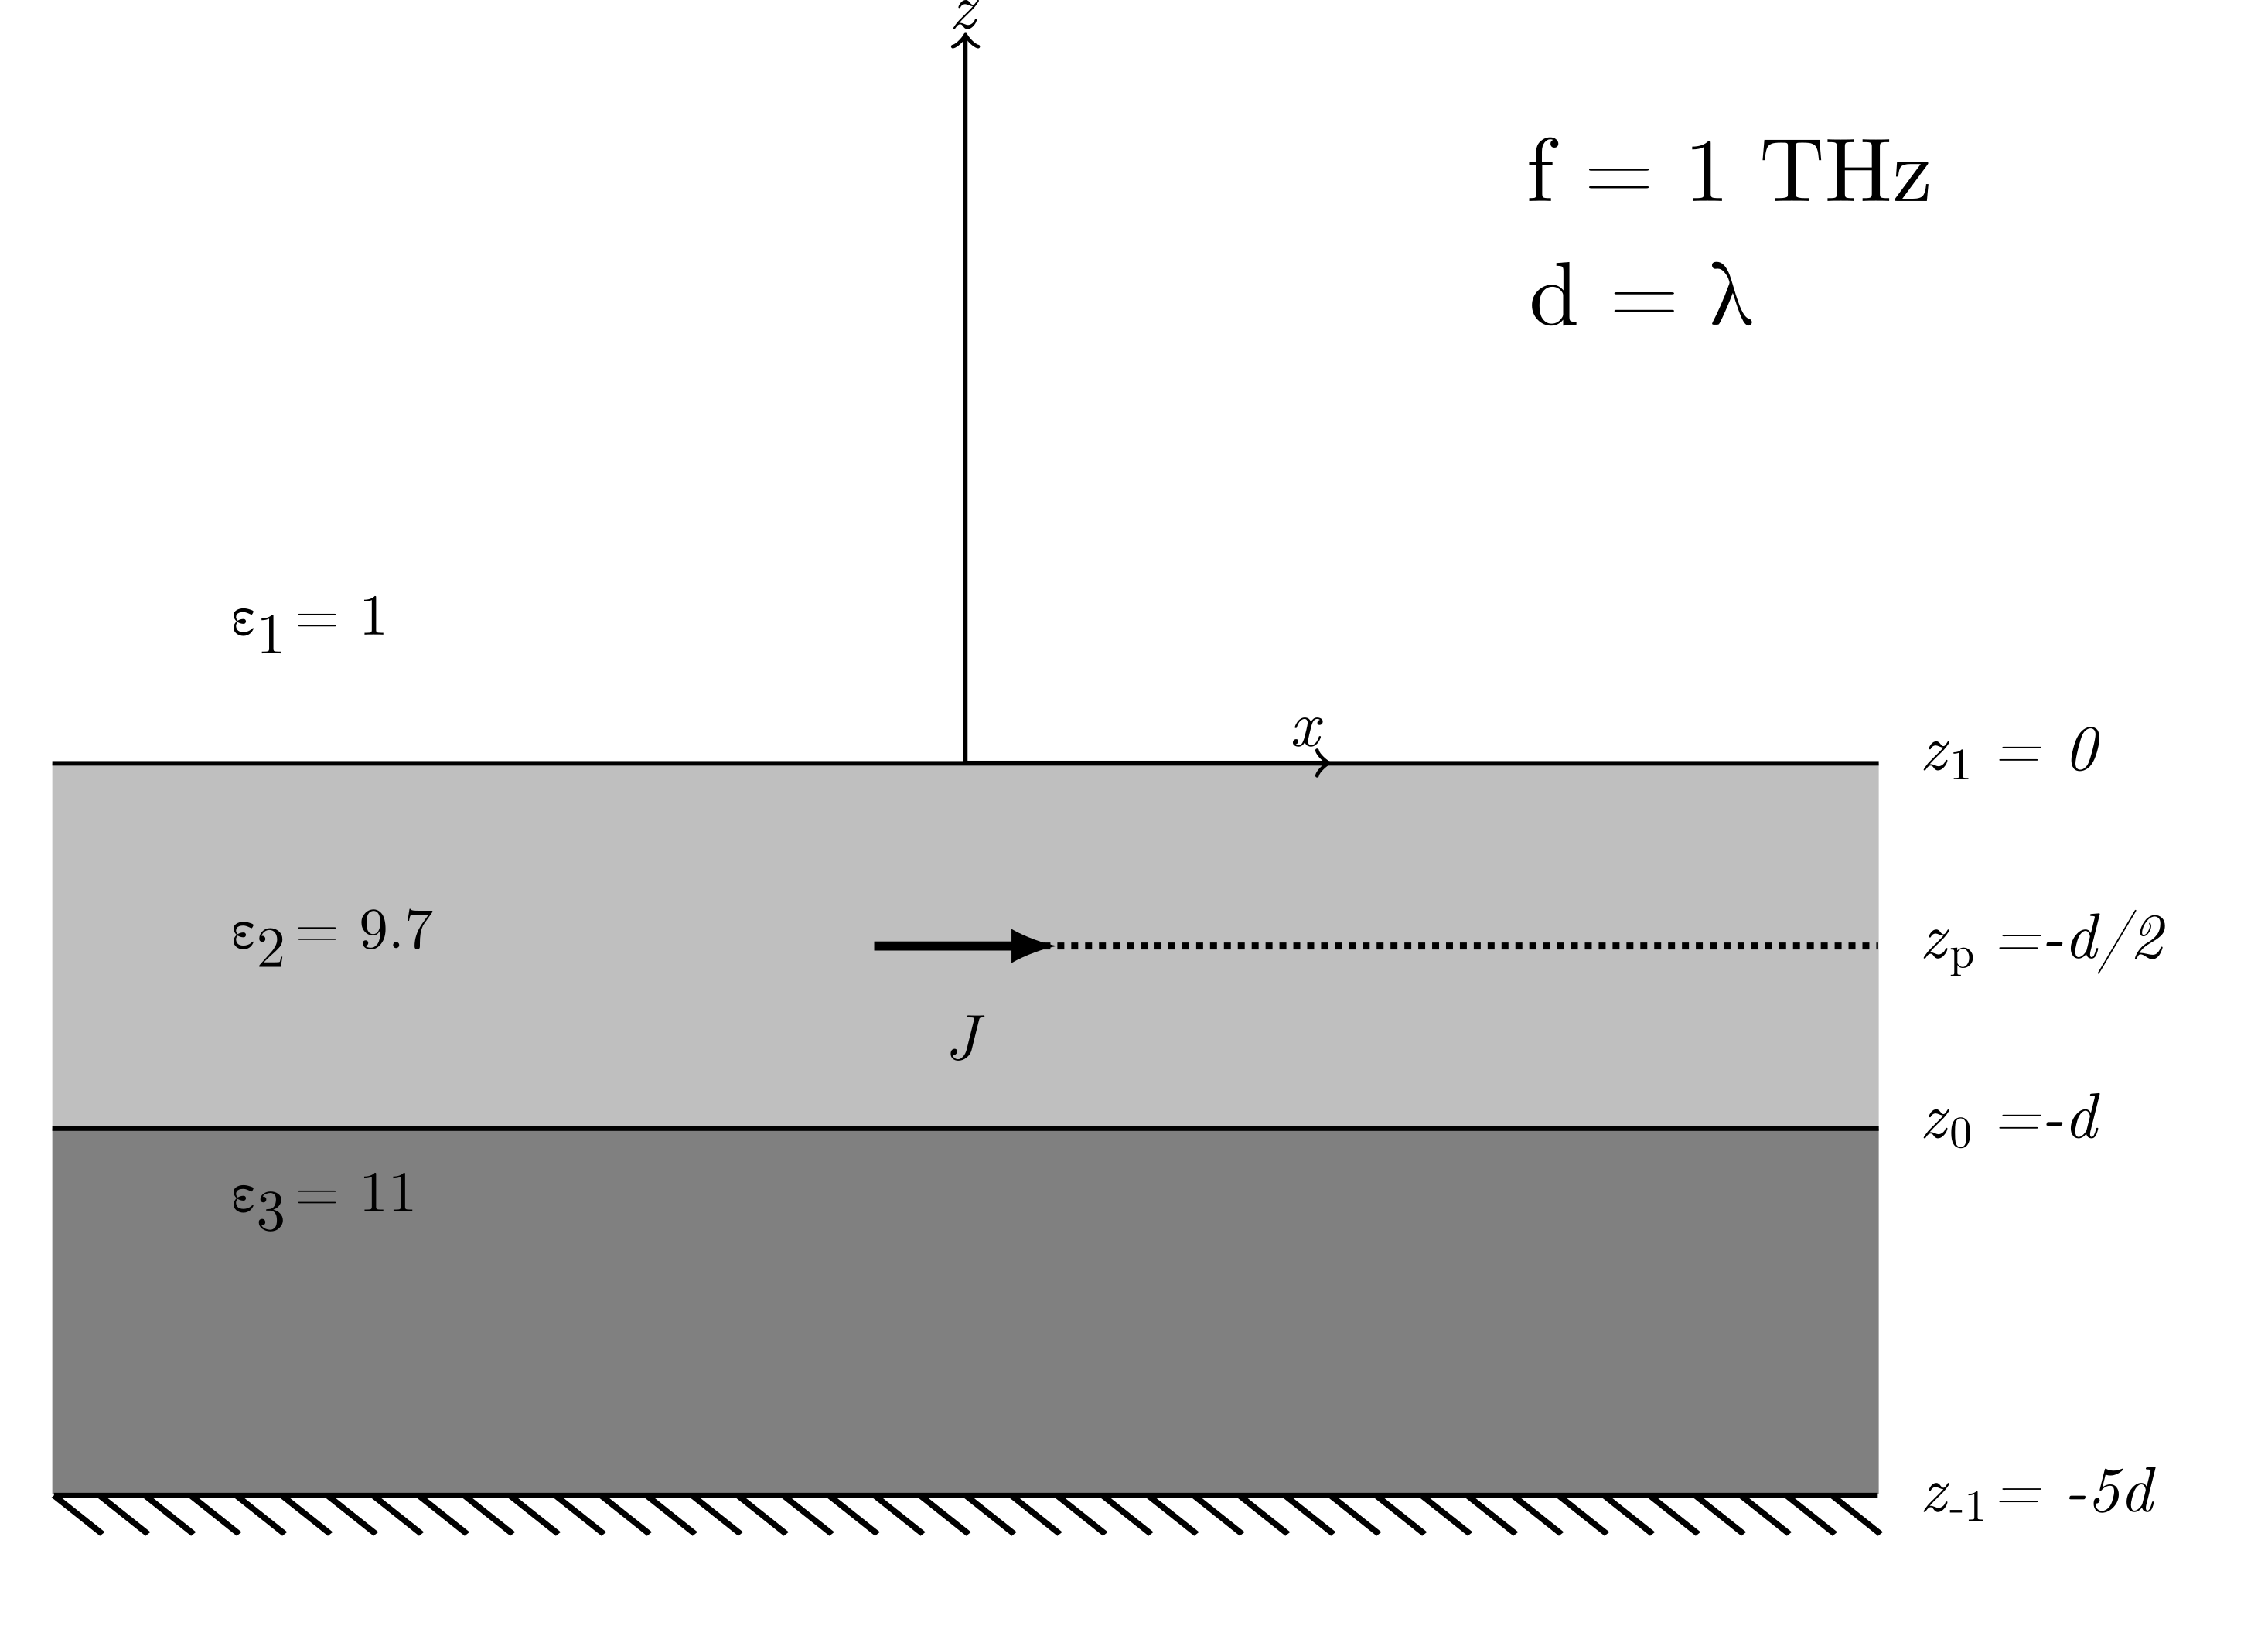
\includegraphics[width=.85\textwidth]{structure_with_PEC_Backing}
  \caption{Structure with PEC base}
  \label{fig:structure_pec}
\end{figure}

$\overleftarrow{\Gamma_2}$ now becomes:

\begin{align}
  \overleftarrow{\Gamma_2} = \frac{{\Gamma_{3,2}} - exp(-4jk_{z3}d)}{ 1 - {\Gamma_{3,2}}exp(-4jk_{z3}d)}
  \label{eq:R_left_pec}
\end{align}

where $\Gamma_{3,2}$ is:
\begin{align}
  \Gamma_{3,2} ={}& \frac{{Z_3} - Z_2}{{Z_3} + Z_2}
  \label{eq:Gamma_32}
\end{align}

The evaluation of $\mathcal D$ with a PEC base is shown in Fig. \ref{fig:zeros_pec}.

\begin{figure}[h!]
  \centering
  \includestandalone[width=.95\textwidth]{zeros_with_pec}
  \caption{Evaluation of (\ref{eq:D}) at computed zeros with PEC}
  \label{fig:zeros_pec}
\end{figure}

A comparison of zeros of two cases in the complex $k_{\rho}$-plane is illustrated in Fig. \ref{fig:comp}

\begin{figure}[h!]
  \centering
  \includestandalone[width=.95\textwidth]{comp}
  \caption{Zeros in the complex plane}
  \label{fig:comp}
\end{figure}
\end{document}
